\chapter{Modelling and Verification in Concurrent Programming}\label{chap:modelling_and_verification_in_concurrent_programming} % (fold)
The importance of models and abstraction for computer science and engineering in particular:
\begin{itemize}
    \item model: rigorous description/representation of program structure and behaviour at a proper level of abstraction, including relevant information, abstracting from non-relevant aspects;
    \item diagrammatical representations for program design;
    \item formal models for program analysis and verification;
\end{itemize}
Defining proper models for \hyperref[def:conc-prog]{Concurrent Programming}:
\begin{itemize}
    \item defining models for the structure and behaviour of concurrent programs abstracting from the low-level details of their actual implementation and realization (\textbf{design});
    \item enabling the possibility to reason about their dynamic behaviour of concurrent programs (\textbf{verification});
\end{itemize}
%
\section{Modelling Concurrent Program Execution using FSP}\label{sec:cp_modelling_concurrent_program_execution_using_fsp} % (fold)
When using \ac{fsp}, processes are the single modelling abstraction for modelling both threads and also shared memory abstractions and mechanisms:
\begin{itemize}
    \item modelling the execution of a sequential program as a \hyperref[def:process]{Process};
    \item modelling the execution of a concurrent program as parallel composition of processes;
    \item modelling shared memory variables as processes as well;
\end{itemize}
%
\subsection{Modelling Using State Diagrams}\label{sub:cp_modelling_using_state_diagrams} % (fold)
The execution of a concurrent program can be formally represented by \textbf{states} and \textbf{transitions} between states.
\begin{definition}{State}{state}
    A \textbf{state} is defined by a tuple consisting of:
    \begin{itemize}
        \item one element of each \hyperref[def:process]{Process} that is a label (\textbf{statement}) from that \hyperref[def:process]{Process};
        \item one element for each global or local variable that is a value whose type is the same as the type of variable;
    \end{itemize}
    There is a transition between two states $s_1$ and $s_2$ if executing a statement in state $s_1$ changes the state of $s_2$: the statement executed must be one of those pointed to by a control pointer is $s_1$.
\end{definition}
\begin{definition}{State Diagram}{state-diagram}
    The \textbf{state diagram} is a \textit{graph} containing all the \textit{reachable states} of the programs; scenarios are represented by directed paths through the state diagram from the initial state.
    \begin{note}
        Cycles represent the possibility of infinite computation in a finite graph
    \end{note}
\end{definition}
\begin{example}{First Trivial Example}{}
    \begin{cimage}
        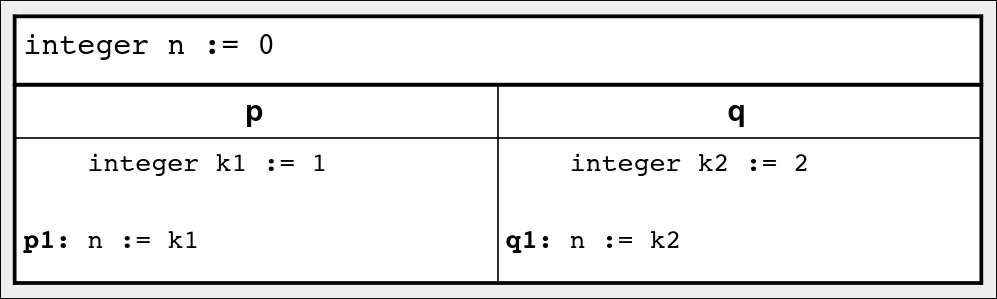
\includegraphics[width=.8\textwidth]{assets/20261013_104513.png}
    \end{cimage}
    \begin{itemize}
        \item each labeled line represents an atomic statement;
        \item each \hyperref[def:process]{Process} has private memory: local variables, such as $k1$ and $k2$;
        \item \hyperref[def:process]{Processes} shares some memory: global variables, such as $n$; 
        \item program execution with 2 scenarios:
            \begin{itemize}
                \item $p1,\,q1 \Rightarrow n$ finally is equal to $2$
                \item $q1,\,p1 \Rightarrow n$ finally is equal to $1$
            \end{itemize}
    \end{itemize}
    The \hyperref[def:state]{State} tuple is $<p,q,n,k1,k2>$ 
    \begin{cimage}
        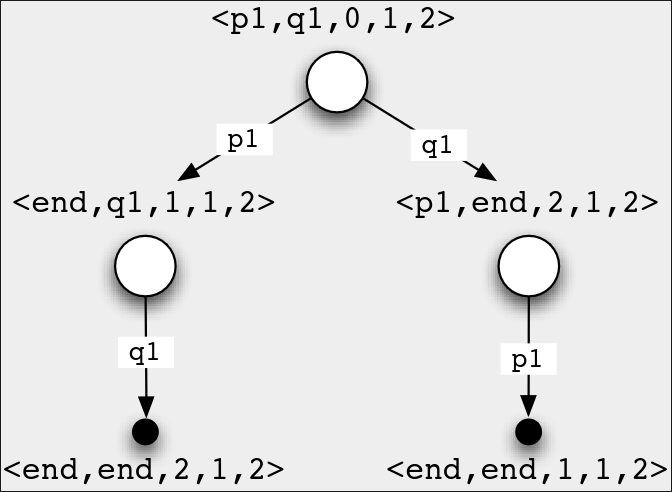
\includegraphics[width=.6\textwidth]{assets/20261013_105048.png}
        \caption{State diagram with 5 \hyperref[def:state]{States} and 2 scenarios}\label{fig:20261013_105048}
    \end{cimage}
\end{example}
\begin{example}{}{}
    \begin{quote}[State diagram? How many scenarios?]
    \end{quote}
    \begin{ctable}{|c|c|}
        \hline
        \textbf{p} & \textbf{q} \\
        \hline
        \textbf{p1:} \texttt{print("p1")} & \textbf{q1:} \texttt{print("q1")} \\
        \textbf{p2:} \texttt{print("p2")} & \textbf{q2:} \texttt{print("q2")} \\
        \hline
    \end{ctable}
    \begin{cimage}
        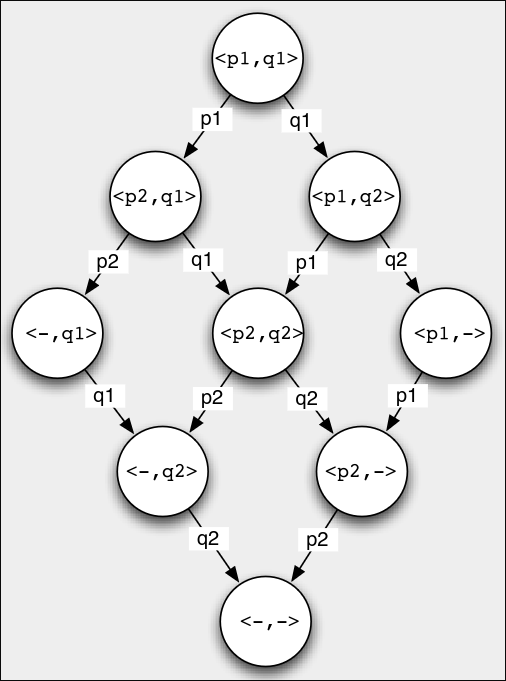
\includegraphics[width=.3\textwidth]{assets/20261013_110029.png}
        $\qquad$
        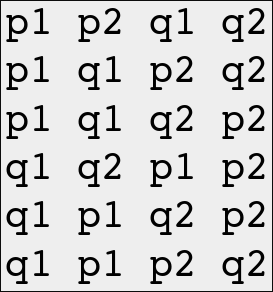
\includegraphics[width=.2\textwidth]{assets/20261013_110052.png}
    \end{cimage}
\end{example}
\subsubsection{Generalizing...}\label{sub:cp_generalizing} % (fold)
The number of scenarios produced by $n$ processes, each having $m_i$ actions is:
\[
    n_s = \dfrac{\pt{\dsum_{i=1}^nm_i}!}{\dprod_{i=1}^n\pt{m_i!}}
\]
\begin{ctable}{r||r|r|r|r|r}
    & $n = 2$ & $3$ & $4$ & $5$ & $6$ \\
    \hline
    \hline
    $m_i$ = $2$ & $6$ & $90$ & $2520$ & $113400$ & $2^{22.8}$ \\
    \hline
    $3$ & $20$ & $1680$ & $2^{18.4}$ & $2^{27.3}$ & $2^{36.9}$ \\
    \hline
    $4$ & $70$ & $34650$ & $2^{25.9}$ & $2^{38.1}$ & $2^{51.5}$ \\
    \hline
    $5$ & $252$ & $2^{19.5}$ & $2^{33.4}$ & $2^{49.1}$ & $2^{66.2}$ \\
    \hline
    $6$ & $924$ & $2^{24.0}$ & $2^{41.0}$ & $2^{60.2}$ & $2^{81.1}$ \\
    \hline
\end{ctable}
% subsubsection Generalizing... (end)
%
\subsubsection{The Importance of being Atomic}\label{sub:cp_the_importance_of_being_atomic} % (fold)
With atomic increment:
\begin{ctable}{|c|c|}
    \hline
    \multicolumn{2}{|l|}{\texttt{integer n := 0}} \\
    \hline
    \textbf{p} & \textbf{q} \\
    \hline
    \textbf{p1:} \texttt{n := n + 1} & \textbf{q1:} \texttt{n := n + 1} \\
    \hline
\end{ctable}
Without an atomic increment:
\begin{ctable}{|l|l|}
    \hline
    \multicolumn{2}{|l|}{\texttt{integer n := 0}} \\
    \hline
    \textbf{p} & \textbf{q} \\
    \hline
    \texttt{integer tmp;} & \texttt{integer tmp;} \\
    \textbf{p1:} \texttt{tmp := n} & \textbf{q1:} \texttt{tmp := n} \\
    \textbf{p2:} \texttt{n := tmp + 1} & \textbf{q2:} \texttt{n := tmp + 1} \\
    \hline
\end{ctable}
\begin{warning}[In the second case, scenarios exist in which the final value of $n$ is $1$]
\end{warning}
\begin{cimage}
    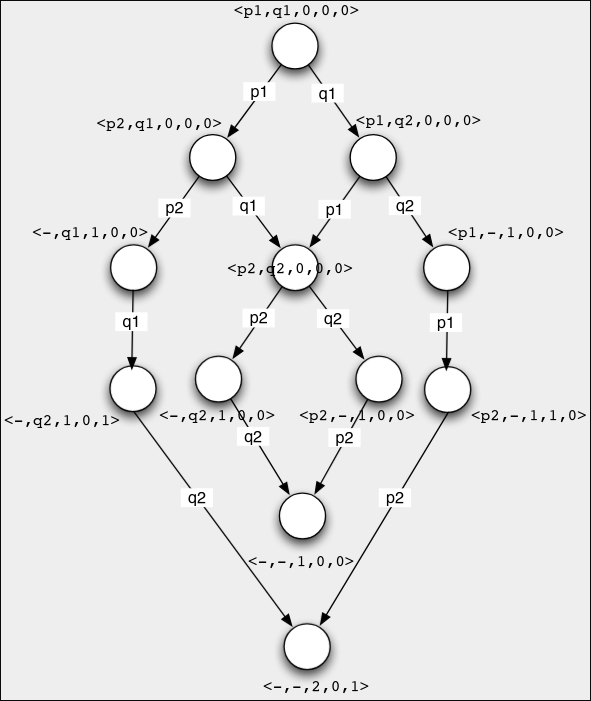
\includegraphics[width=.4\textwidth]{assets/20261013_113712.png}
    \caption{Diagram with 12 states, only 2 scenarios over 6 have final $n = 2$}\label{fig:20261013_113712}
\end{cimage}
% subsubsection The Importance of being Atomic (end)
%
\subsubsection{Non-Atomic Structures}\label{sub:cp_non_atomic_structures} % (fold)
The notion of ``atomic'' can be referred not only to actions, but also to data structures.
\begin{definition}{Atomic Data Object}{atomic-object}
    A data object is defined \textbf{atomic} if it can be in a finite number of \hyperref[def:state]{States} equals to the number of values that it can assume, operations change atomically that state.
\end{definition}
\begin{quote}
    Typically, primitive data type in concurrent languages are atomic
    \begin{warning}[Not always]
        Abstract data types composed by multiple simpler data objects are typically \textbf{non-atomic}
    \end{warning}
\end{quote}
In that case for the ADT (or more generally data object) it is possible to identify two basic types of \hyperref[def:state]{States}: \textbf{internal} and \textbf{external}.
\begin{definition}{Internal State}{int-state}
    An \textbf{internal state} is meaningful for who defines the data object (class)
\end{definition}
\begin{definition}{External State}{ext-state}
    An \textbf{external state} is meaningful for who uses the data object (class)
\end{definition}
The correspondence among internal and external states is \textit{partial}: there exists internal state which have no correspondent external state.
\begin{definition}{Consistent State}{consistent-state}
    Internal state which have a corresponded external state are defined \textbf{consistent}
\end{definition}
Then, the execution of an operation on an ADT can go through states that are \textbf{not \hyperref[def:consistent-state]{consistent}}
\begin{note}
    This is not a problem in the case of sequential programming, thanks to information hiding
    \begin{critical}
        Conversely, it is a problem in the case of concurrent programming: it can happen that a process would work on an object while the object is in an inconsistent state, since a \hyperref[def:process]{Process} that are operating on it.
    \end{critical}
\end{note}
\begin{remark}{}{}
    It is necessary to introduce proper mechanisms that would guarantee that processes work on data objects that are always in states that are \hyperref[def:consistent-state]{consistent}
\end{remark}
% subsubsection Non Atomic Structures (end)
%
\subsubsection{Cyclic Processes}\label{sub:cp_cyclic_processes} % (fold)
$p$ and $q$ processes cycling on a condition:
\begin{ctable}{|l|l|}
    \hline
    \multicolumn{2}{|l|}{\texttt{integer n := 1}} \\
    \hline
    \textbf{p} & \textbf{q} \\
    \hline
    \textbf{p1:} \texttt{while (n < 1)} & \textbf{q1:} \texttt{while (n >= 0)} \\
    \textbf{p2:} \texttt{n := n + 1} & \textbf{q2:} \texttt{n := n - 1} \\
    \hline
\end{ctable}
\begin{note}[Analysis]
    \begin{itemize}
        \item state diagram?
        \item construct a scenario in which the loop in $p$ executes exactly one;
        \item construct a scenario in which the loop in $p$ executes exactly three times;
        \item construct a scenario in which both loops execute infinitely often;
    \end{itemize}
\end{note}
\begin{cimage}
    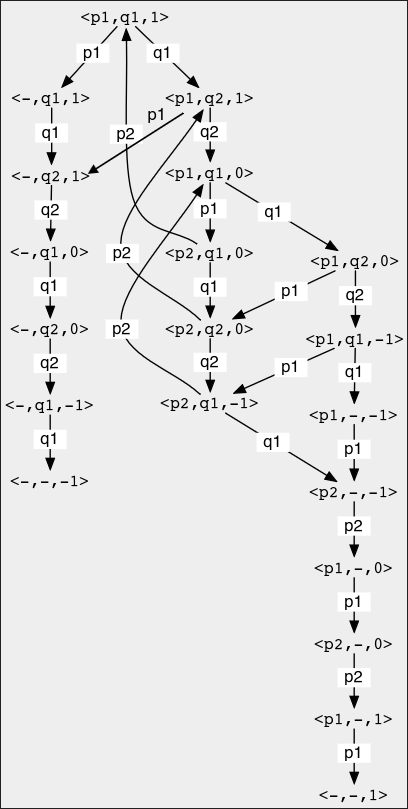
\includegraphics[width=.4\textwidth]{assets/20261013_122811.png}
    \caption{The state diagram}\label{fig:20261013_122811}
\end{cimage}
% subsubsection Cyclic Processes (end)
% subsection Modelling Using State Diagrams (end)
%
% section Modelling Concurrent Program Execution using FSP (end)
%
\section{The Critical Section Problem}\label{sec:cp_the_critical_section_problem} % (fold)
Introduced by Dijkstra, the \hyperref[sub:an_critical_sections]{Critical Section} problem can be considered one of the most important and well-studied problem in \hyperref[def:conc-prog]{Concurrent Programming}, in the context of \hyperref[def:process]{Process} competition.
\begin{theorem}{Problem Definition}{cs-problem}
    $N$ processes, each executing in an infinite loop as a sequence of statements that can be divided in $2$ subsequences: the \hyperref[sub:an_critical_sections]{Critical Section} and the \textit{non-critical} section.
    \begin{codeblock}{}
    P[1..n]:
    loop {
        <non-critical section>
        entry (or pre-) protocol
        <critical section>
        exit (or post-) protocol
        <non-critical section>
    }
    \end{codeblock}
    \begin{note}
        Each \hyperref[sub:an_critical_sections]{Critical Section} is typically a sequence of statements that access some shared object
    \end{note}
\end{theorem}
The problem is intended to model a system that performs complex computation, but occasionally need to access data or resources that are shared by several \hyperref[def:process]{Processes}.
\begin{example}{}{}
    A check-in-kiosk at an airport, accessing to a central database of passengers
\end{example}
%
\subsection{Critical Sections Properties}\label{sub:cp_critical_sections_properties} % (fold)
Our task is to design \textit{entry and exit protocols} that satisfy the following properties:
\begin{itemize}
    \item \textbf{mutual exclusion}, statements from the \hyperref[def:crit-sec]{Critical Sections} of two or more \hyperref[def:process]{Processes} must not be interleaved;
    \item \textbf{freedom from deadlock}, if some \hyperref[def:process]{Processes} are trying to enter their \hyperref[def:crit-sec]{Critical Sections}, then one of them must eventually succeed;
    \item \textbf{freedom from individual starvation}, if any \hyperref[def:process]{Process} tries to enter their \hyperref[def:crit-sec]{Critical Section} then that \hyperref[def:process]{Process} must eventually succeed (\textbf{bounded waiting property});
\end{itemize}
\begin{note}
    Any proposed solution must satisfy also the \textbf{progress property} for the  \hyperref[def:crit-sec]{Critical Section}: once a process starts to execute the statements of its critical section, it must eventually finish
    \begin{critical}[The non-critical section need not to progress]
    \end{critical}
\end{note}
% subsection Critical Sections Properties (end)
%
\subsection{Critical Section Solution}\label{sub:cp_critical_section_solution} % (fold)
The \hyperref[th:cs-problem]{critical section problem} can be easily solved by using basic mechanisms such as \textit{semaphores} or \textit{locks}, that must be provided by the concurrent machine.
\begin{note}
    In this section we focus instead on a purely algorithmic solution without using high-level mechanism, but solely basic atomic statements (e.g. load and store)
\end{note}
%
\subsubsection{CS for Two Processes}\label{sub:cp_cs_for_two_processes} % (fold)
First we analyse the problem considering $2$ \hyperref[def:process]{Processes} $P$ and $Q$ sharing some global variables.
% -- sample cs problems table ---
\begin{ctable}{|l|l|}
    \hline
    \multicolumn{2}{|l|}{\textbf{Critical Section Problem}} \\
    \hline
    \multicolumn{2}{|l|}{Global Variables} \\
    \hline
    \multicolumn{2}{|l|}{} \\
    \multicolumn{2}{|c|}{
        \begin{ntable}{|l|l|}
            \hline
            \textbf{p} & \textbf{q} \\
            \hline
            \texttt{Local Variables} & \texttt{Local Variables} \\
            & \\
            \texttt{loop forever} & \texttt{loop forever} \\
            \texttt{    non-critical section} & \texttt{    non-critical section} \\
            \texttt{    pre-protocol} & \texttt{    pre-protocol} \\
            \texttt{    critical section} & \texttt{    critical section} \\
            \texttt{    post-protocol} & \texttt{    post-protocol} \\
            \hline
        \end{ntable}
    } \\
    \multicolumn{2}{|l|}{} \\
    \hline
\end{ctable}
% -- sample cs problems table ---
\begin{note}
    The protocols may require local or global variables, we assume that no variables used in the \hyperref[def:crit-sec]{Critical Section} and non-critical section \red{are used} in the protocols
\end{note}
\begin{remark}{First Attempt}{first-algo}
    Let's consider a first possible solution
    \begin{ctable}{|l|l|}
        \hline
        \multicolumn{2}{|l|}{\textbf{First Attempt}} \\
        \hline
        \multicolumn{2}{|l|}{Integer turn $\leftarrow 1$} \\
        \hline
        \multicolumn{2}{|l|}{} \\
        \multicolumn{2}{|c|}{
            \begin{ntable}{|l|l|}
                \hline
                \textbf{p} & \textbf{q} \\
                \hline
                & \\
                \texttt{loop forever} & \texttt{loop forever} \\
                \textbf{p1:} \texttt{non-critical section} & \textbf{q1:} \texttt{non-critical section} \\
                \textbf{p2:} \texttt{await turn = 1} & \textbf{q2:} \texttt{await turn = 2} \\
                \textbf{p3:} \texttt{critical section} & \textbf{q3:} \texttt{critical section} \\
                \textbf{p4:} \texttt{turn $\leftarrow 2$} & \textbf{q4:} \texttt{turn $\leftarrow 1$} \\
                \hline
            \end{ntable}
        } \\
        \multicolumn{2}{|l|}{} \\
        \hline
    \end{ctable}
    The statement \texttt{\textbf{await} turn $\leftarrow 1$} is an implementation independent notation for a statement that waits until the \textit{condition} \texttt{turn = 1} becomes true.
    \begin{note}
        This can be implemented by a busy-wait loop that does nothing until the condition is true
        \begin{warning}[Inefficient]
        \end{warning}
    \end{note}
    \begin{outerproof}{Checking Correctness}{}
        In order to prove the \textbf{correctness} of the solution we construct the state diagram of the \hyperref[def:conc-prog]{Concurrent Program}: the algorithm must satisfy the \hyperref[sub:cp_critical_sections_properties]{Critical Sections Properties}.
        \emptyln{}
        To check correctness properties is only necessary to examine the set of reachable states and the transitions among them.
        States are a triple $<p_i,q_j,\texttt{turn}>$ where:
        \begin{itemize}
            \item $p_i$ is the current control pointer for process $P$;
            \item $q_j$ is the current control pointer for process $Q$;
            \item \texttt{turn} is the content of the variable;
        \end{itemize}
        The diagram is constructed incrementally starting from the initial state and considering what the potential states are.
        \emptyln{}
        Describing the mutual exclusion property is important to check if it holds the set of all accessible states does not contain a state of the form:
        \[
            <p_3,q_3,\_>
        \]
        Next we express properties in \hyperref[sub:an_ltl_temporal_operators]{LTL}:
        \begin{itemize}
            \item \textit{mutual exclusion property}: $\cbox \neg\pt{p_3 \wedge q_3}$
            \item \textit{freedom of starvation properties}:
                \begin{itemize}
                    \item $\cbox\pt{p_3\to\dm p_4}$
                    \item $\cbox\pt{q_3\to\dm q_4}$
                \end{itemize}
        \end{itemize}
    \end{outerproof}
    \begin{note}[Are properties satisfied?]
        \begin{itemize}
            \item the \textbf{mutual exclusion} is satisfied: there are no scenarios including states of the kind $<p_2,q_2,\_$;
            \item the \textbf{freedom of deadlock} is satisfied: if some processes are trying to enter the \hyperref[def:crit-sec]{CS} (executing the $\texttt{await}$), then one eventually succeeds;
            \item the \textbf{freedom of starvation} is \textbf{not satisfied}: a process that wants to enter in \hyperref[def:crit-sec]{CS} (pre-protocol) can starve while waiting a process which engaged an infinite loop inside its non-critical section (where there is no progress property);
                \begin{note}
                    Turn function as permission resource to enter the \hyperref[def:crit-sec]{Critical Section}, if the process holding the permission remains indefinitely in its non-critical section, the other \hyperref[def:process]{Process} will never receive the resource and will never enter its \hyperref[def:crit-sec]{Critical Section}: both processes sets and tests a single global variable, if one process dies the other is blocked
                \end{note}
        \end{itemize}
    \end{note}
\end{remark}
\begin{remark}{Second Attempt}{}
    We introduce separate \texttt{want} variables whose purpose is to make it explicit and observable the intention of a \hyperref[def:process]{Process} to enter in its \hyperref[def:crit-sec]{Critical Section}.
    \begin{ctable}{|l|l|}
        \hline
        \multicolumn{2}{|l|}{\textbf{Second Attempt}} \\
        \hline
        \multicolumn{2}{|l|}{\texttt{boolean wantp $\leftarrow$false}} \\
        \multicolumn{2}{|l|}{\texttt{boolean wantq $\leftarrow$false}} \\
        \hline
        \multicolumn{2}{|l|}{} \\
        \multicolumn{2}{|c|}{
            \begin{ntable}{|l|l|}
                \hline
                \textbf{p} & \textbf{q} \\
                \hline
                & \\
                \texttt{loop forever} & \texttt{loop forever} \\
                \textbf{p1:} \texttt{non-critical section} & \textbf{q1:} \texttt{non-critical section} \\
                \textbf{p2:} \texttt{await wantq = false} & \textbf{q2:} \texttt{await wantp = false} \\
                \textbf{p3:} \texttt{wantp = true} & \textbf{q3:} \texttt{wantq = true} \\
                \textbf{p4:} \texttt{critical section} & \textbf{q4:} \texttt{critical section} \\
                \textbf{p5:} \texttt{wantp $\leftarrow$false} & \textbf{q5:} \texttt{wantq $\leftarrow$false} \\
                \hline
            \end{ntable}
        } \\
        \multicolumn{2}{|l|}{} \\
        \hline
    \end{ctable}
    \begin{itemize}
        \item \textbf{mutual exclusion}: $\cbox\neg\pt{p_4\wedge q_4}$
        \item \textbf{freedom from starvation}: $\cbox\pt{\pt{p_1\to\dm p_2} \wedge \pt{q_1\to\dm q_2}}$
    \end{itemize}
    \begin{outerproof}{Checking Correctness}{}
        By constructing the \hyperref[def:state-diagram]{State Diagram} it is simple to see that the mutual exclusion property is not satisfied: the state $<p_3,p_3,\texttt{true}, \texttt{true}>$ is reachable.
        \begin{note}
            The problem is due to the non-atomicity of the pre-protocol and post-protocol
        \end{note}
        \emptyln{}
    \end{outerproof}
\end{remark}
\begin{remark}{Third Attempt}{}
    Previous problem can be solved by considering the await statement part of the \hyperref[def:crit-sec]{Critical Section} and moving the assignment before the await.
    \begin{ctable}{|l|l|}
        \hline
        \multicolumn{2}{|l|}{\textbf{Third Attempt}} \\
        \hline
        \multicolumn{2}{|l|}{\texttt{boolean wantp $\leftarrow$false}} \\
        \multicolumn{2}{|l|}{\texttt{boolean wantq $\leftarrow$false}} \\
        \hline
        \multicolumn{2}{|l|}{} \\
        \multicolumn{2}{|c|}{
            \begin{ntable}{|l|l|}
                \hline
                \textbf{p} & \textbf{q} \\
                \hline
                & \\
                \texttt{loop forever} & \texttt{loop forever} \\
                \textbf{p1:} \texttt{non-critical section} & \textbf{q1:} \texttt{non-critical section} \\
                \textbf{p2:} \texttt{wantp $\leftarrow$ true} & \textbf{q2:} \texttt{wantq $\leftarrow$ true} \\
                \textbf{p3:} \texttt{await lwantq} & \textbf{q3:} \texttt{await lwantp} \\
                \textbf{p4:} \texttt{critical section} & \textbf{q4:} \texttt{critical section} \\
                \textbf{p5:} \texttt{wantp $\leftarrow$false} & \textbf{q5:} \texttt{wantq $\leftarrow$false} \\
                \hline
            \end{ntable}
        } \\
        \multicolumn{2}{|l|}{} \\
        \hline
    \end{ctable}
    \begin{outerproof}{Correctness}{}
        The mutual exclusion problem is \textbf{solved}, however the solution suffer of \textbf{livelocks}: there are scenarios in which both \hyperref[def:process]{Processes} are trying to enter in their \hyperref[def:crit-sec]{Critical Section}, but neither will ever do.
    \end{outerproof}
\end{remark}
\begin{remark}{Fourth Attempt}{fourth-algo}
    \hyperref[def:deadlock]{Deadlock} occurs when both \hyperref[def:process]{Processes} simultaneously insist on entering their \hyperref[def:crit-sec]{Critical Section}: the next step to solve the problem is requiring a \hyperref[def:process]{Process} to give up its intention to enter its \hyperref[def:crit-sec]{Critical Section} if it discovers that it is contending with the other \hyperref[def:process]{Process}.
    \begin{ctable}{|l|l|}
        \hline
        \multicolumn{2}{|l|}{\textbf{Fourth Attempt}} \\
        \hline
        \multicolumn{2}{|l|}{\texttt{boolean wantp $\leftarrow$false}} \\
        \multicolumn{2}{|l|}{\texttt{boolean wantq $\leftarrow$false}} \\
        \hline
        \multicolumn{2}{|l|}{} \\
        \multicolumn{2}{|c|}{
            \begin{ntable}{|l|l|}
                \hline
                \textbf{p} & \textbf{q} \\
                \hline
                & \\
                \texttt{loop forever} & \texttt{loop forever} \\
                \textbf{p1:} \texttt{non-critical section} & \textbf{q1:} \texttt{non-critical section} \\
                \textbf{p2:} \texttt{wantp $\leftarrow$ true} & \textbf{q2:} \texttt{wantq $\leftarrow$ true} \\
                \textbf{p3:} \texttt{while wantq} & \textbf{q3:} \texttt{while wantp} \\
                \textbf{p4:} \texttt{   wantp $\leftarrow$false} & \textbf{q4:} \texttt{   wantq $\leftarrow$false} \\
                \textbf{p5:} \texttt{   wantp $\leftarrow$true} & \textbf{q5:} \texttt{   wantq $\leftarrow$true} \\
                \textbf{p6:} \texttt{critical section} & \textbf{q6:} \texttt{critical section} \\
                \textbf{p7:} \texttt{wantp $\leftarrow$false} & \textbf{q7:} \texttt{wantq $\leftarrow$false} \\
                \hline
            \end{ntable}
        } \\
        \multicolumn{2}{|l|}{} \\
        \hline
    \end{ctable}
    \begin{note}[But livelock can also occur in this case]
    \end{note}
\end{remark}
% subsubsection CS for Two Processes (end)
% subsection Critical Section Solution (end)
%
\subsection{Dekker's Algorithm}\label{sub:cp_dekker_s_algorithm} % (fold)
The problem can be solved with a simple variation of the \hyperref[rem:fourth-algo]{Fourth Attempt} requiring the \textit{right to insist} on entering -- instead of the right to enter -- is explicitly passed between the \hyperref[def:process]{Processes} by means of the variable \texttt{turn}.
\begin{note}
    Dekker's algorithm for solving \hyperref[sec:cp_the_critical_section_problem]{The Critical Section Problem} can be then considered a \textbf{combination} of the \hyperref[rem:first-algo]{First Attempt} and the \hyperref[rem:fourth-algo]{Fourth Attempt}
\end{note}
\begin{ctable}{|l|l|}
    \hline
    \multicolumn{2}{|l|}{\textbf{Dekker's Algorithm}} \\
    \hline
    \multicolumn{2}{|l|}{\texttt{boolean wantp $\leftarrow$false}} \\
    \multicolumn{2}{|l|}{\texttt{boolean wantq $\leftarrow$false}} \\
    \multicolumn{2}{|l|}{\texttt{integer turn $\leftarrow 1$}} \\
    \hline
    \multicolumn{2}{|l|}{} \\
    \multicolumn{2}{|c|}{
        \begin{ntable}{|l|l|}
            \hline
            \textbf{p} & \textbf{q} \\
            \hline
            & \\
            \texttt{loop forever} & \texttt{loop forever} \\
            \textbf{p1:} \texttt{non-critical section} & \textbf{q1:} \texttt{non-critical section} \\
            \textbf{p2:} \texttt{wantp $\leftarrow$ true} & \textbf{q2:} \texttt{wantq $\leftarrow$ true} \\
            \textbf{p3:} \texttt{while wantq} & \textbf{q3:} \texttt{while wantp} \\
            \textbf{p4:} \texttt{   if turn = 2} & \textbf{q4:} \texttt{   if turn = 1} \\
            \textbf{p5:} \texttt{   wantp $\leftarrow$false} & \textbf{q5:} \texttt{     wantq $\leftarrow$false} \\
            \textbf{p6:} \texttt{   await turn = 1} & \textbf{q6:} \texttt{     await turn = 1} \\
            \textbf{p7:} \texttt{   wantp $\leftarrow$true} & \textbf{q7:} \texttt{      wantq $\leftarrow$true} \\
            \textbf{p8:} \texttt{critical section} & \textbf{q8:} \texttt{critical section} \\
            \textbf{p8:} \texttt{turn $\leftarrow2$} & \textbf{q9:} \texttt{turn $\leftarrow1$} \\
            \textbf{p10:} \texttt{wantp $\leftarrow$false} & \textbf{q10:} \texttt{wantq $\leftarrow$false} \\
            \hline
        \end{ntable}
    } \\
    \multicolumn{2}{|l|}{} \\
    \hline
\end{ctable}
\begin{itemize}
    \item \textbf{mutual exclusion}: $\cbox\neg\pt{p_8 \wedge q_8}$
    \item \textbf{freedom from starvation}: $\cbox\pt{\pt{p_2\to\dm p_8} \wedge \pt{q_2\to\dm q_8}}$
\end{itemize}
%
\subsubsection{Peterson's Algorithm}\label{sub:cp_peterson_s_algorithm} % (fold)
Other solutions have been proposed through time, improving \hyperref[sub:cp_dekker_s_algorithm]{Dekker's Algorithm}.
Peterson's solution is more concise, by collapsing the two await statements into one with a compound condition.
\begin{ctable}{|l|l|}
    \hline
    \multicolumn{2}{|l|}{\texttt{boolean wantp := false}} \\
    \multicolumn{2}{|l|}{\texttt{boolean wantq := false}} \\
    \multicolumn{2}{|l|}{\texttt{integer turn := 1}} \\
    \hline
    \multicolumn{2}{|l|}{} \\
    \multicolumn{2}{|c|}{
        \begin{ntable}{|l|l|}
            \hline
            \textbf{p} & \textbf{q} \\
            \hline
            & \\
            \texttt{loop forever} & \texttt{loop forever} \\
            \textbf{p1:} \texttt{non-critical section} & \textbf{q1:} \texttt{non-critical section} \\
            \textbf{p2:} \texttt{wantp := true} & \textbf{q2:} \texttt{wantq := true} \\
            \textbf{p3:} \texttt{turn := 2} & \textbf{q3:} \texttt{turn := 1} \\
            \textbf{p4:} \texttt{await !wantq || turn = 1} & \textbf{q4:} \texttt{await !wantp || turn = 2} \\
            \textbf{p5:} \texttt{critical section} & \textbf{q5:} \texttt{critical section} \\
            \textbf{p6:} \texttt{wantp := false} & \textbf{q6:} \texttt{wantq := false} \\
            \hline
        \end{ntable}
    } \\
    \multicolumn{2}{|l|}{} \\
    \hline
\end{ctable}
% subsubsection Peterson's Algorithm (end)
%
\subsubsection{Bakery Algorithm (Tie-Breaker)}\label{sub:cp_bakery_algorithm_tie_breaker} % (fold)
An alternative solution to \hyperref[def:crit-sec]{Critical Section} problem for $N$-\hyperref[def:process]{Process} accounts for introducing a \textit{ticket} to establish the turn of a \hyperref[def:process]{Process}.
\begin{ctable}{|l|}
    \hline
    $N$-process solution for CS with tickets \\
    \hline
    \texttt{int num := 1} \\
    \texttt{int next := 1} \\
    \texttt{turn[1:n] := [0,0,0,...]} \\
    \hline
    \textbf{p[i]} \\
    \hline
    \texttt{loop forever} \\
    \textbf{p1:} \texttt{NCS} \\
    \textbf{p2:} \texttt{< turn[i] := num; num := num + 1 >} \\
    \textbf{p3:} \texttt{await turn[i] = next} \\
    \textbf{p4:} \texttt{CS} \\
    \textbf{p5:} \texttt{next := next + 1} \\
    \hline
\end{ctable}
\begin{note}[Potential shortcomings]
    Arithmetic overflow for \texttt{turn} and \texttt{num}: monotonically growing
\end{note}
% subsubsection Bakery Algorithm (Tie-Breaker) (end)
% subsection Dekker's Algorithm (end)
%
\subsection{Compound Atomic Statements}\label{sub:cp_compound_atomic_statements} % (fold)
\hyperref[sub:cp_dekker_s_algorithm]{Dekker's Algorithm} works on any architecture, providing just load and store as atomic statements.
Actually, the algorithm and -- more generally -- \hyperref[sec:cp_the_critical_section_problem]{The Critical Section Problem} and mutual exclusion problems can be greatly simplified if we can exploit more complex atomic statements: directly provided by the \hyperref[def:conc-machine]{Concurrent Machine}.
\begin{note}
    Main examples are \texttt{test-and-set}, \texttt{exchange}, \texttt{fetch-and-add}, \texttt{compare-and-swap}
    \begin{warning}
        \texttt{test-and-set} is an atomic statement defined as the execution of the two following statements with no possibility of interleaving
        \begin{codeblock}{}
        test-and-set (x,r):
        < r := x, x := 1 >
        \end{codeblock}
    \end{warning}
    \begin{note}[A commonly used notation for specifying atomicity is to put angled bracket around the group of statements]
    \end{note}
\end{note}
\begin{example}{Critical Section with Test-and-Set}{}
    \begin{ctable}{|l|l|}
        \hline
        \multicolumn{2}{|l|}{\texttt{integer lock := 0}} \\
        \hline
        \textbf{p} & \textbf{q} \\
        \hline
        \texttt{integer was\_locked} & \texttt{integer was\_locked} \\
                                     & \\
        \texttt{loop forever} & \texttt{loop forever} \\
        \textbf{p1:} \texttt{NCS} & \textbf{q1:} \texttt{NCS}  \\
        \texttt{    repeat} & \texttt{    repeat} \\
        \textbf{p2:} \texttt{test\_and\_set(lock, was\_locked)} & \textbf{q2:} \texttt{test\_and\_set(lock, was\_locked)} \\
        \textbf{p3:} \texttt{until was\_locked} & \textbf{q3:} \texttt{until was\_locked} \\
        \textbf{p4:} \texttt{CS} & \textbf{q4:} \texttt{CS} \\
        \textbf{p5:} \texttt{lock := 0} & \textbf{q5:} \texttt{lock := 0} \\
        \hline
    \end{ctable}
\end{example}
%
\subsubsection{Locks}\label{sub:cp_locks} % (fold)
By exploiting \hyperref[sub:cp_compound_atomic_statements]{Compound Atomic Statements} we can easily realize basic \textbf{lock} mechanism:
\begin{itemize}
    \item simple solution for \hyperref[sec:cp_the_critical_section_problem]{The Critical Section Problem};
    \item protecting \hyperref[def:crit-sec]{Critical Section} of code;
\end{itemize}
\begin{note}
    Two stages/atomic operations:
    \begin{itemize}
        \item \textbf{acquiring} the lock;
        \item \textbf{releasing} the lock;
    \end{itemize}
\end{note}
\begin{ctable}{|l|l|}
    \hline
    \multicolumn{2}{|l|}{\texttt{lock sharedlock;}} \\
    \hline
    \textbf{p} & \textbf{q} \\
    \hline
    \texttt{loop forever} & \texttt{loop forever} \\
    \textbf{p1:} \texttt{NCS} & \textbf{q1:} \texttt{NCS}  \\
    \textbf{p2:} \texttt{acquire(sharedlock)} & \textbf{q2:} \texttt{acquire(sharedlock)} \\
    \textbf{p3:} \texttt{CS} & \textbf{q3:} \texttt{CS} \\
    \textbf{p4:} \texttt{release(sharedlock)} & \textbf{q4:} \texttt{release(sharedlock)} \\
    \hline
\end{ctable}
% subsubsection Locks (end)
% subsection Compound Atomic Statements (end)
% section The Critical Section Problem (end)
% chapter Modelling and Verification in Concurrent Programming (end)
